\documentclass[../main.tex]{subfiles}
\begin{document}

Bayesian regression with gaussian errors, like ordinary least-square regression is quite sensitive to outliers\cite{rousseeuw2005robust}.
To increase outlier robustness, a Bayesian regression model with Student-T errors is more effective\cite{gelman2013bayesian}.
This is the first model which while being relatively straightforward is quite effective in several real-world usecases.

\begin{equation}
y \sim StudentT(\nu, \mu, \sigma)
\end{equation}
Here, $\nu$ is the degrees of freedom parameter.
As $\nu$ approaches $\inf$, the distribution approaches normal.
Here we choose prior for $\nu$ as:
$$
   \nu \sim Gamma(shape=2, scale=10)
$$
$\mu$ is the mean of the regression and is given by:
$$
\mu = \alpha + \beta * X
$$
$\sigma$ is the variance of the $StudentT$ distribution and has a prior:
$$
\sigma \sim  Exponential(scale_\sigma)
$$
And $\alpha, \beta, X$ are sampled from:
$$
\alpha \sim Normal(0, scale_\alpha), \quad \beta \sim Normal(0, scale_\beta), \quad X \sim Normal(0, 10)
$$

\subsection{Data Generation}
PPLBench generates all the data internally.
This allows for a more customizable way to evaluate the PPL implementations of the model.
In this case, to test the robustness of the model implementations, we generate data by sampling the alphas and betas from the $\sigma = [10, 11]$ tails of the distribution.
A total of $2N = 2000$ data points were generated, where each point being generated from a sample drawn for these  tails of parameter distributions.
We use half of the generated data as evidence for the model implementations to facilitate convergence of sampling process.
The other half are used to compute the posterior predictive log-likelihood of the parameter samples.
\begin{table}[h]
 \caption{Hyperpriors for Robust Regression Model}
  \centering
  \begin{tabular}{lll}              \\
    \cmidrule(r){1-3}
    Hyperprior      & Value     & Notes  \\
    \midrule
    $scale_\alpha$    & 10        & Variance of the Normal prior of $\alpha$    \\
    $scale_\beta$     & 2.5       & Variance of the Normal prior of $\beta$     \\
    $scale_\sigma$    & 1         & Scale of Exponential prior of $\sigma$      \\
    Tails             & [10, 11]    & Tails of prior distributions              \\
    \bottomrule
  \end{tabular}
  \label{tab:table_RR}
\end{table}
\subsection{PPL Implementations}
The robust regression model was implemented in Stan and Jags PPLs, with the help of PyStan\cite{PyStan} and PyJAGS\cite{PyJAGS} libraries for interface.
The compilation and inference times were recorded.
The configuration of hyperpriors is listed in table\ref{tab:table_RR}.
One noteworthy difference between the two would be that Jags uses Gibbs sampler while Stan uses NUTS HMC.
This difference will be important when we analyze the results.

\begin{figure}[h]
  \centering
  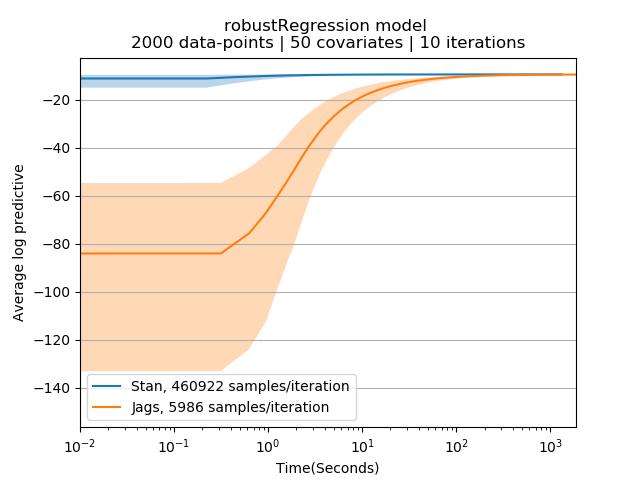
\includegraphics[width=150mm]{analysis_robust_regression.png}
  \caption{Posterior convergence behaviour of Jags and Stan for Robust Regression model}
  \label{fig:fig2}
\end{figure}

\subsection{Results}
Figure \ref{fig:fig1} shows the comparative performance without considering the inference time.
From the figure, we can make the following observations:
\begin{itemize}
\item Both implementations converge to the same posterior predictive log-likelihood given enough time.
\item Without considering compile time, Stan is both faster to converge as well has a much lower time per sample.
\item Stan’s NUTS inference starts sampling from relatively high log-likelihood space  and hence converges much quicker than Jags’ Gibbs sampler, which has a much slower convergence.
\end{itemize}

\end{document}
